\subsection{Meal schedule}

The two figures in this section, \cref{MealScheduleList} and \cref{MealScheduleBar}, displays two design ideas for the meal schedule aspect of the program. In \cref{MealScheduleList} 2 sketches are shown, and they indicate the first idea that were thought of in the context of design. The left sketch show the meal schedule for a week, and the right show the meals scheduled on a specific day. In \cref{MealScheduleBar} the screen that is going to be the design of the program is shown. The sketches of \cref{MealScheduleList} have been combined to make the final sketch shown in \cref{MealScheduleBar}

\begin{figure}[H]
	\centering
    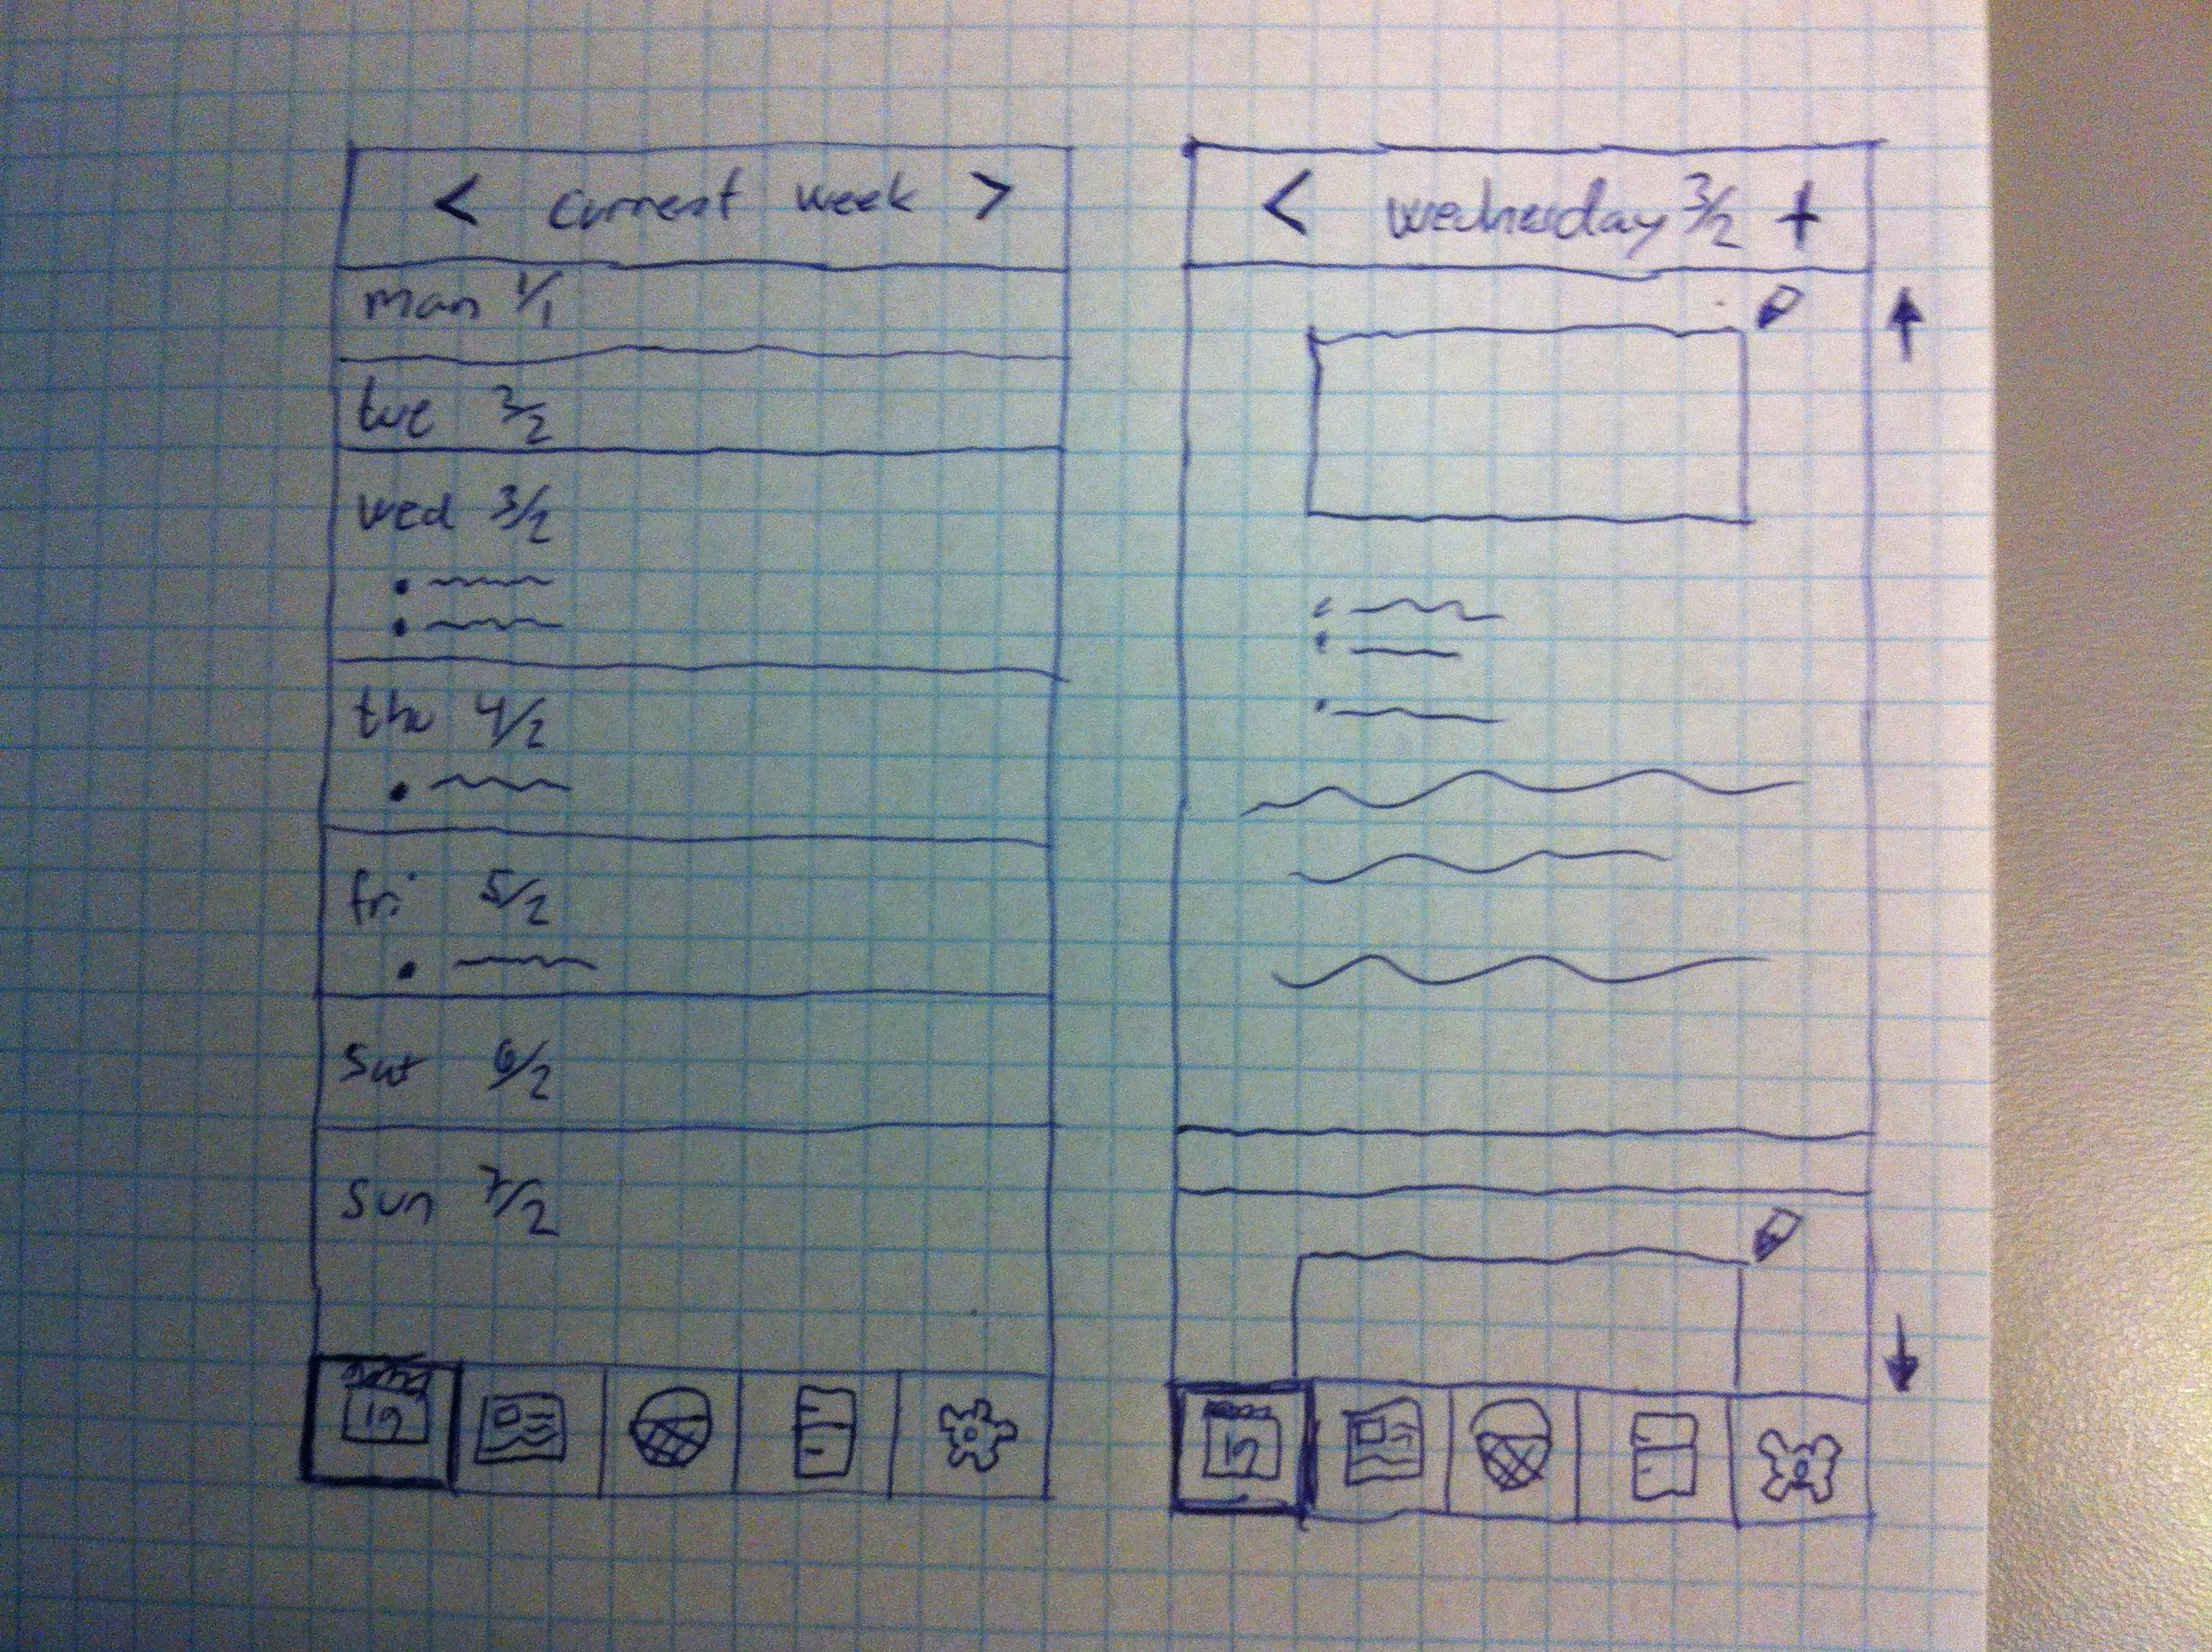
\includegraphics[width=0.5\textwidth]{Grafik/FoodPlanner/FinalMealScheduleSketch1}
	\caption{The left screen shows 7 days of a specific week and the right screen shows scheduled meals on a specific day.}
	\label{MealScheduleList}
\end{figure}

\subsection{First draft: Week schedule} \label{FirstDraftWeekSchedule}

Looking at the first draft of the week schedule, \cref{MealScheduleList}, there are two elements to look at:

\begin{itemize}
    \item Navigation bar
    \item Schedule
\end{itemize}

The navigation is placed at the top of the screen, because the sides of a screen, and especially top and bottom, are places that users tend to look to find navigation, and since the bottom is already used by the navigation of the entire program, it is the natural choice to place it at the top. This also gives some symmetry to the program, because as mentioned, the bottom is filled by the navigation bar for the entire program.

The schedule element of the sketch, shows seven days of the schedule. Seven is chosen because it is a week, and the availability to plan a week ahead is useful if the user plans the same day of the week, and plans the rest of the weeks. Each day of the schedule would show the name of the recipe scheduled, the date of the day, and some of the ingredients needed in the recipe. If the user chose to click a day, the day would expand, and more information about the scheduled meal would appear.

\subsection{First draft: Specific recipe screen} \label{FirstDraftSpecificRecipeScreen}

The specific recipe screen seen in \cref{MealScheduleList} show the recipes that are scheduled for a specific day. The sketch consist of 2 elements, not counting the general elements:

\begin{itemize}
    \item Navigation bar
    \item Scheduled recipes
\end{itemize}

The navigation bar works in some ways like the navigation bar described in \cref{FirstDraftWeekSchedule}, the differences are; you can not go to the next day from the navigation bar, and you are able to add another recipe by clicking the plus icon. 

The scheduled recipes is a list of all the scheduled recipes for that day. The list is ordered in a downwards fashion, so the user can go through all the scheduled recipes by scrolling through. If the user either want to change the recipe, or delete it, the user can click on the pencil icon, which means edit. A recipe consists of all the information about a recipe, this means picture, ingredients list and the list of instructions.

\subsection{Final design}

The final design of the MealPlan screen, can be seen in figure: \cref{MealScheduleBar}. The screen consists of 2 elements, not counting the general design elements:

\begin{itemize}
    \item Week navigation
    \item Scheduled recipes.
\end{itemize}

The week navigation is placed as a bar, in the left edge of the screen. This bar show 7 days at a time, and have arrows going up and down to go through weeks. The reason for arrows and not the scrolling, is that by clicking a day, the scheduled recipes shown will change, so it is easy to misclick, if scrolling by swiping up and down is done, therefore buttons are used.
The icons of the week navigation show the date, and a number. The number indicates the amount of recipes scheduled on the day, if no meals are scheduled, no number will be shown. 

The scheduled recipes, work as described in section \ref{FirstDraftSpecificRecipeScreen}.

\begin{figure}[H]
	\centering
    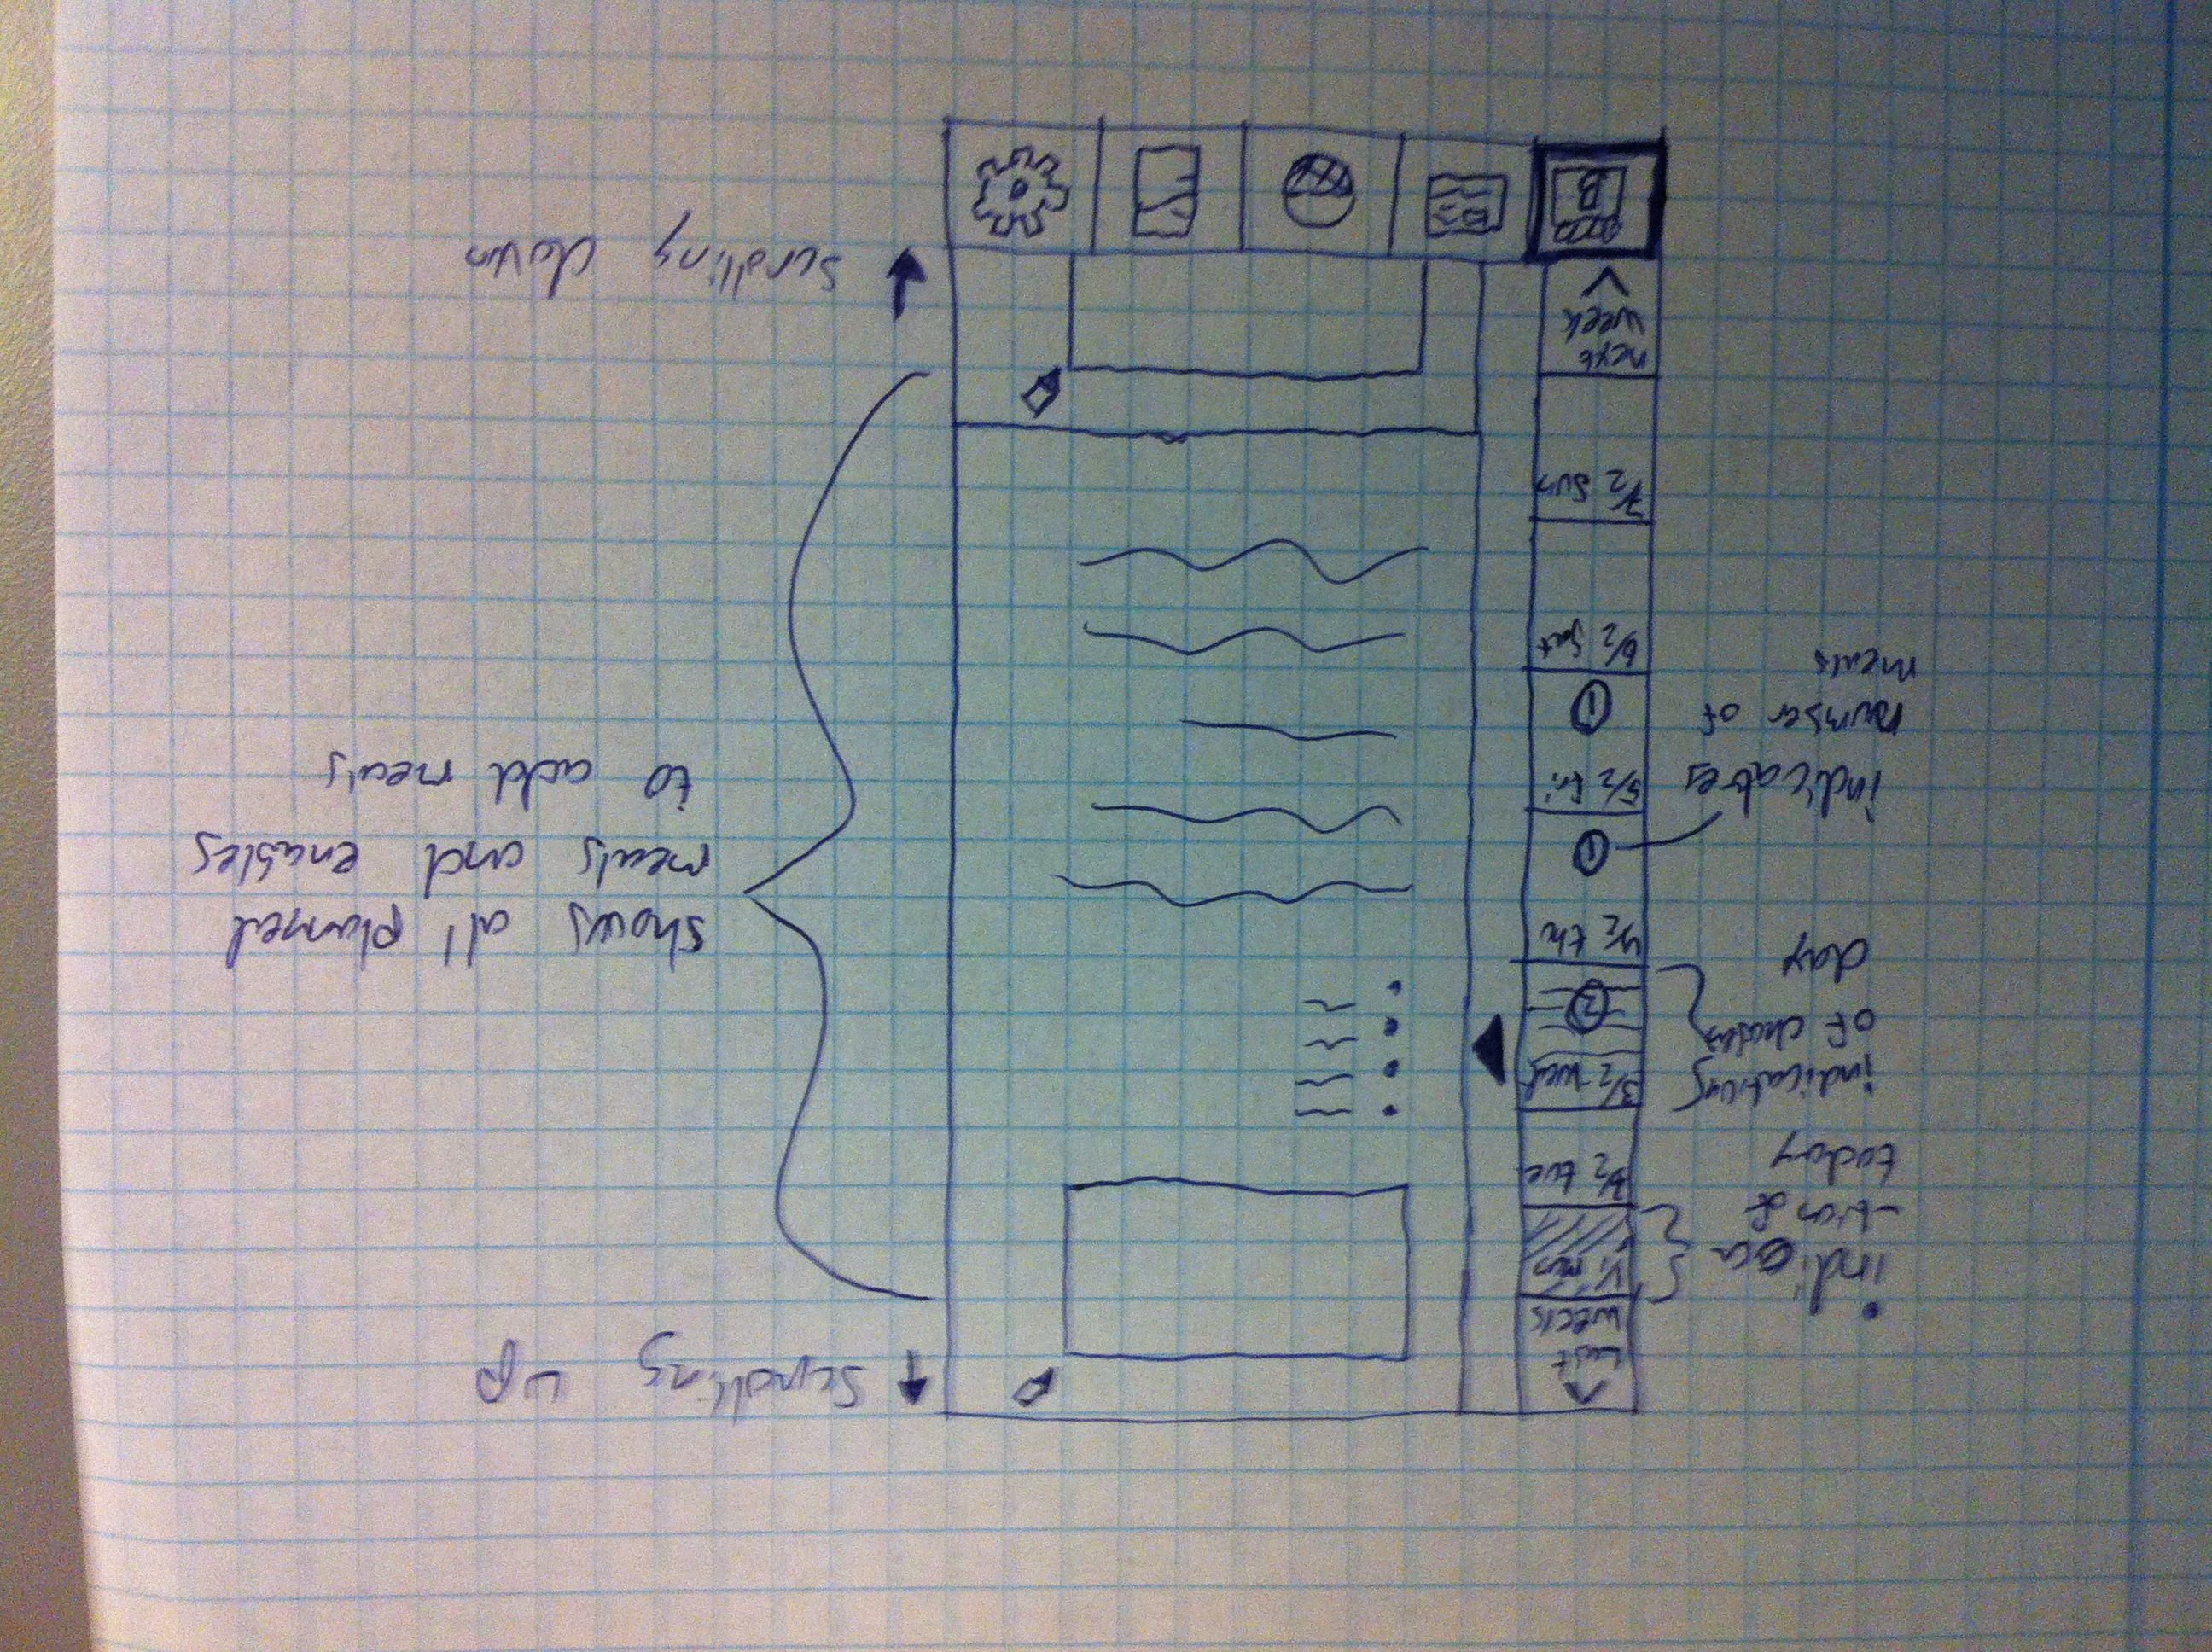
\includegraphics[width=0.5\textwidth]{Grafik/FoodPlanner/FinalMealScheduleSketch2}
	\caption{This sketch merges both of the screens above into one screen with the weeks on the left bar and the scheduled meals as a list on the right side of the screen.}
	\label{MealScheduleBar}
\end{figure}

